\documentclass[svgnames,table,,aspectratio=169]{beamer}
%\documentclass[svgnames,table,handout,aspectratio=129]{beamer}
\usepackage{hhline}
\usepackage{etoolbox}
\usepackage{tikz}
\usepackage{mathtools}
\usepackage{amssymb}
%\usepackage{/usr/lib64/R/share/texmf/Sweave}
\usepackage{polynom}
\usepackage{qrcode}
\usepackage{ulem}

%\input{latexdefinitions}
\definecolor{georgiaRed}{RGB}{100,0,00}
\definecolor{mediumGray}{gray}{0.6}



\usetheme{Frankfurt}%
%\usetheme{Warsaw}%
%\useoutertheme{smoothbars}


%\usecolortheme{seagull}
\usecolortheme{beaver}
\logo{\includegraphics[height=.125in]{ugaLogo}}

% Note that the colour definitions are given in the latexDefinitions
% file.
\setbeamercolor{palette primary}{fg=georgiaRed,bg=white}
\setbeamercolor{palette secondary}{fg=georgiaRed,bg=white}
\setbeamercolor{palette tertiary}{fg=georgiaRed,bg=white}
\setbeamercolor{palette quaternary}{bg=mediumGray,fg=black}
\setbeamercolor{block title}{fg=white,bg=georgiaRed}
\setbeamercolor{block body}{fg=black,bg=black!10}
\setbeamercolor{titlelike}{bg=georgiaRed,fg=white} % parent=palette quaternary}

% Define the variable to determine whether or not the clicker quizzes
% are visible in the resulting output.
\newtoggle{clicker}
\toggletrue{clicker}
%\togglefalse{clicker}


% To display a lecture uncomment out the "includeonly" line below to
% match the name of the file. You do not have to do anything with the
% lecture line below and can leave it commented out. It is in place
% because at one time we had multiple lectures within a file, but that
% has been changed.



\mode<presentation>{
  \setbeamercovered{invisible}
  \setbeameroption{hide notes}
}

\mode<handout>{
 
  \usepackage{pgfpages}
  %\pgfpagesuselayout{4 on 1}[letterpaper, border shrink=5mm]
  \pgfpagesuselayout{resize to}[letterpaper,border shrink=5mm]
  \setbeameroption{show notes}


  %\pgfpagesphysicalpageoptions{logical pages=2,physical
  %height=\pgfpageoptionheight,physical width=\pgfpageoptionwidth}
  % Set up the pages for notes.
  % This idea and some code came from
  % http://www.guidodiepen.nl/2009/07/creating-latex-beamer-handouts-with-notes/



  \pgfpagesdeclarelayout{3 on 1 with notes} {
    \edef\pgfpageoptionheight{11in} %\the\paperheight}
    \edef\pgfpageoptionwidth{8.5in} %\the\paperwidth}
    \edef\pgfpageoptionborder{0pt}
  }

  {

	\AtBeginDocument{
      \newbox\notesbox
      \setbox\notesbox=\vbox{
        \hsize=\paperwidth
        \vskip-2.5cm\hskip-5cm\vbox{
          \textcolor{light-gray}{\hrule width 12.6cm\vskip0.5cm}
          \textcolor{light-gray}{\hrule width 12.6cm\vskip0.5cm}
          \textcolor{light-gray}{\hrule width 12.6cm\vskip0.5cm}
          \textcolor{light-gray}{\hrule width 12.6cm\vskip0.5cm}
          \textcolor{light-gray}{\hrule width 12.6cm\vskip0.5cm}
          \textcolor{light-gray}{\hrule width 12.6cm\vskip0.5cm}
          \textcolor{light-gray}{\hrule width 12.6cm\vskip0.5cm}
          \textcolor{light-gray}{\hrule width 12.6cm\vskip0.5cm}
          \textcolor{light-gray}{\hrule width 12.6cm\vskip0.5cm}
          \textcolor{light-gray}{\hrule width 12.6cm\vskip0.5cm}
          \textcolor{light-gray}{\hrule width 12.6cm\vskip0.5cm}
          \textcolor{light-gray}{\hrule width 12.6cm\vskip0.5cm}
          \textcolor{light-gray}{\hrule width 12.6cm\vskip0.5cm}
          \textcolor{light-gray}{\hrule width 12.6cm\vskip0.5cm}
          \textcolor{light-gray}{\hrule width 12.6cm\vskip0.5cm}
          \textcolor{light-gray}{\hrule width 12.6cm\vskip0.5cm}
          \textcolor{light-gray}{\hrule width 12.6cm\vskip0.5cm}
          \textcolor{light-gray}{\hrule width 12.6cm\vskip0.5cm}
          \textcolor{light-gray}{\hrule width 12.6cm\vskip0.5cm}

          \vspace*{-9.75cm}
          \textcolor{light-gray}{\rule[-1.0cm]{1pt}{9.25cm}\hskip0.5cm}
          \textcolor{light-gray}{\rule[-1.0cm]{1pt}{9.25cm}\hskip0.5cm}
          \textcolor{light-gray}{\rule[-1.0cm]{1pt}{9.25cm}\hskip0.5cm}
          \textcolor{light-gray}{\rule[-1.0cm]{1pt}{9.25cm}\hskip0.5cm}
          \textcolor{light-gray}{\rule[-1.0cm]{1pt}{9.25cm}\hskip0.5cm}
          \textcolor{light-gray}{\rule[-1.0cm]{1pt}{9.25cm}\hskip0.5cm}
          \textcolor{light-gray}{\rule[-1.0cm]{1pt}{9.25cm}\hskip0.5cm}
          \textcolor{light-gray}{\rule[-1.0cm]{1pt}{9.25cm}\hskip0.5cm}
          \textcolor{light-gray}{\rule[-1.0cm]{1pt}{9.25cm}\hskip0.5cm}
          \textcolor{light-gray}{\rule[-1.0cm]{1pt}{9.25cm}\hskip0.5cm}
          \textcolor{light-gray}{\rule[-1.0cm]{1pt}{9.25cm}\hskip0.5cm}
          \textcolor{light-gray}{\rule[-1.0cm]{1pt}{9.25cm}\hskip0.5cm}
          \textcolor{light-gray}{\rule[-1.0cm]{1pt}{9.25cm}\hskip0.5cm}
          \textcolor{light-gray}{\rule[-1.0cm]{1pt}{9.25cm}\hskip0.5cm}
          \textcolor{light-gray}{\rule[-1.0cm]{1pt}{9.25cm}\hskip0.5cm}
          \textcolor{light-gray}{\rule[-1.0cm]{1pt}{9.25cm}\hskip0.5cm}
          \textcolor{light-gray}{\rule[-1.0cm]{1pt}{9.25cm}\hskip0.5cm}
          \textcolor{light-gray}{\rule[-1.0cm]{1pt}{9.25cm}\hskip0.5cm}
          \textcolor{light-gray}{\rule[-1.0cm]{1pt}{9.25cm}\hskip0.5cm}
          \textcolor{light-gray}{\rule[-1.0cm]{1pt}{9.25cm}\hskip0.5cm}

        }

      }

    \pgfpagesphysicalpageoptions
    {%
      logical pages=6,%
      physical height=\pgfpageoptionheight,%
      physical width=\pgfpageoptionwidth,%
      last logical shipout=3%
    }
    
    \pgfpageslogicalpageoptions{1}
    {%
      border shrink=\pgfpageoptionborder,%
      resized width=.5\pgfphysicalwidth,%
      resized height=.33\pgfphysicalheight,%
      center=\pgfpoint{.25\pgfphysicalwidth}{.82\pgfphysicalheight}%
    }%
    \pgfpageslogicalpageoptions{2}
    {%
      border shrink=\pgfpageoptionborder,%
      resized width=.5\pgfphysicalwidth,%
      resized height=.33\pgfphysicalheight,%
      center=\pgfpoint{.25\pgfphysicalwidth}{.47\pgfphysicalheight}%
    }%
    \pgfpageslogicalpageoptions{3}
    {%
      border shrink=\pgfpageoptionborder,%
      resized width=.5\pgfphysicalwidth,%
      resized height=.33\pgfphysicalheight,%
      center=\pgfpoint{.25\pgfphysicalwidth}{.17\pgfphysicalheight}%
    }%	
	\pgfpageslogicalpageoptions{4}
    {%
      border shrink=\pgfpageoptionborder,%
      resized width=.5\pgfphysicalwidth,%
      resized height=.33\pgfphysicalheight,%
      center=\pgfpoint{.85\pgfphysicalwidth}{.82\pgfphysicalheight},%
      copy from=4
    }%
    \pgfpageslogicalpageoptions{5}
    {%
      border shrink=\pgfpageoptionborder,%
      resized width=.5\pgfphysicalwidth,%
      resized height=.33\pgfphysicalheight,%
      center=\pgfpoint{.85\pgfphysicalwidth}{.47\pgfphysicalheight},%
      copy from=5
    }%
    \pgfpageslogicalpageoptions{6}
    {%
      border shrink=\pgfpageoptionborder,%
      resized width=.5\pgfphysicalwidth,%
      resized height=.33\pgfphysicalheight,%
      center=\pgfpoint{.85\pgfphysicalwidth}{.17\pgfphysicalheight},%
      copy from=6
    }%
    
      \pgfpagesshipoutlogicalpage{4}\copy\notesbox
      \pgfpagesshipoutlogicalpage{5}\copy\notesbox
      \pgfpagesshipoutlogicalpage{6}\copy\notesbox
    }
  }

  \pgfpagesuselayout{3 on 1 with notes}

}

\setbeamercolor{upper separation line head}{bg=red}
\setbeamercolor{headline}{bg=red}
\setbeamertemplate{headline}
{%
\begin{beamercolorbox}{section in head/foot}
\insertsectionnavigationhorizontal{.75\textwidth}{}{}
\hfill \insertpagenumber /\insertdocumentendpage
\end{beamercolorbox}%
}
\setbeamercolor{section number projected}{bg=red,fg=black}
\setbeamercolor{subsection number projected}{bg=red,fg=black}
%\setbeamercolor{frametitle}{bg=lightgray,fg=black}

\setbeamertemplate{itemize item}{\color{georgiaRed}$\blacklozenge$}
\setbeamertemplate{itemize subitem}{\color{georgiaRed}$\blacktriangleright$}

\newcommand{\dotfield}[2]{%
  \begin{tikzpicture}[y=0.25cm, x=0.25cm,font=\sffamily]
    \foreach \y in {0,...,#2} {
      \foreach \x in {0,...,#1} {
        \draw[fill=georgiaRed,opacity=0.1] (\x,\y)  circle [radius=0.03em];
      }
    }
  \end{tikzpicture}
}

\newcommand{\twoByTwo}[4]{%
  \left[
    \begin{array}{rr}
      #1 & #2 \\
      #3 & #4 \\
    \end{array}
  \right]
}

\newcommand{\threeByThree}[9]{%
  \left[
    \begin{array}{rrr}
      #1 & #2 & #3 \\
      #4 & #5 & #6 \\
      #7 & #8 & #9
    \end{array}
  \right]
}

\newcommand{\columnVector}[1]{%
  \left[
    \begin{array}{r}
    #1                           
    \end{array}
  \right]
}


\begin{document}



\author{\textsc{T. Alli$^{a}$, K. Black$^{a}$}}
\institute{$^a$Department of Mathematics, University of Georgia, GA}
\subject{Linear Algebra}
\keywords{Linear Transformation, Vectors, Matrices, Linear Algebra}

%\lecture{Partial Fractions}{partial-fractions}
%\section{Rational Functions}

\title{Section 3.1: Matrix Transformations}
\subtitle{matrix Multiplication As A Function}


\date{} % {\today}

\begin{frame}
  \titlepage
\end{frame}

\begin{frame}{Outline}
  \tableofcontents
\end{frame}


\section{Goals}

\begin{frame}{Goals}

  A matrix transformation is a function defined by a matrix multiplied
  by a vector.
  
  \begin{itemize}
  \item Provide a geometric interpretation of a matrix transformation.
  \item Identify a matrix transformation as a shear, reflection,
    rotation, or a projection.
  \item Determine the domain, co-domain, and range of a matrix transformation.
  \end{itemize}

\end{frame}

\section{Matrix Transformation}

\begin{frame}{Matrix/Vector Multiplication}

  We have already seen matrix/vector multiplication,
  \begin{eqnarray*}
    A\vec{x} & = & \left[ \vec{a}_1 ~ \vec{a}_2 \cdots \vec{a}_n  \right] \vec{x} \\
             & = & x_1 \vec{a}_1 + x_2 \vec{a}_2 + \cdots + x_n \vec{a}_n.
  \end{eqnarray*}

  Given a vector, $\vec{x}$, we have a rule to turn it into something
  else. This can be used to define a function.

\end{frame}

\begin{frame}{Matrix Transformation}

  \begin{block}{Definition: Matrix Transformation}
    A matrix transformation is defined by the function
    \begin{eqnarray*}
      F\left(\vec{x}\right) & = & A\vec{x} \\
                            & = & \left[ \vec{a}_1 ~ \vec{a}_2 \cdots \vec{a}_n  \right] \vec{x} \\
                            & = & x_1 \vec{a}_1 + x_2 \vec{a}_2 + \cdots + x_n \vec{a}_n.
    \end{eqnarray*}

  \end{block}

  Note: If $A$ is an $m\times n$ matrix then it takes a vector in
  ${\mathbb R}^n$ and returns a vector in ${\mathbb R}^m$.
    

\end{frame}


\begin{frame}{What Does It Mean?}

  \begin{itemize}
  \item We will explore this idea throughout the course, and it will
    be a source of continuing \sout{pain} \textit{joy}.
  \item There are multiple things that a matrix transformation can do.
  \item There are combinations of these things.
  \item What we will do here:
    \begin{itemize}
    \item Introduce the basic idea.
    \item Examine some examples.
    \item Try to get a basic idea of what can happen.
    \item Start the exploration of this idea.
    \end{itemize}
  \end{itemize}
  
\end{frame}

\section{Basic Idea}

\begin{frame}{Basic Idea}

  We have a matrix transformation defined by $A\vec{u}$ where $A$ is a
  matrix.

  \center
  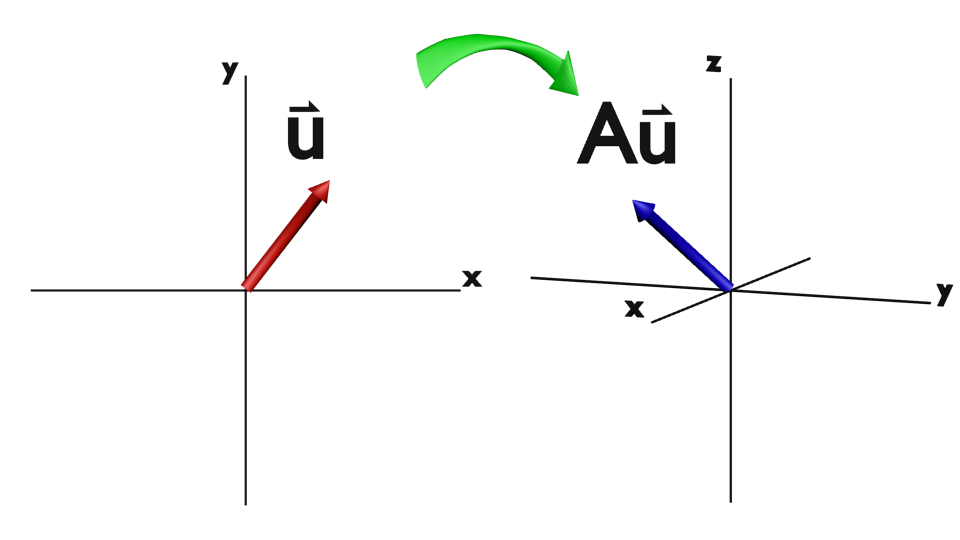
\includegraphics[height=0.8\textheight]{transofrmationOneVector}
  
\end{frame}

\begin{frame}{Questions}

  \begin{itemize}
  \item Where do the inputs come from?
  \item What is the collection of all possible inputs?
  \item Where do the outputs go?
  \item What is the collection of all possible outputs?
  \item What is the relationship between one input and one output?
  \end{itemize}
  
\end{frame}

\section{Examples}

\begin{frame}{Example: Projection}
  \begin{columns}[T]
    \column{0.25\textwidth}
  Define a matrix transformation by
  \begin{eqnarray*}
    P: & & {\mathbb R}^3 \rightarrow {\mathbb R}^3, \\
    P\vec{x} & = & \threeByThree{0}{0}{0}{0}{1}{0}{0}{0}{1}\columnVector{x\\y\\z}.
  \end{eqnarray*}

  \column{0.75\textwidth}
  \uncover<2->{
    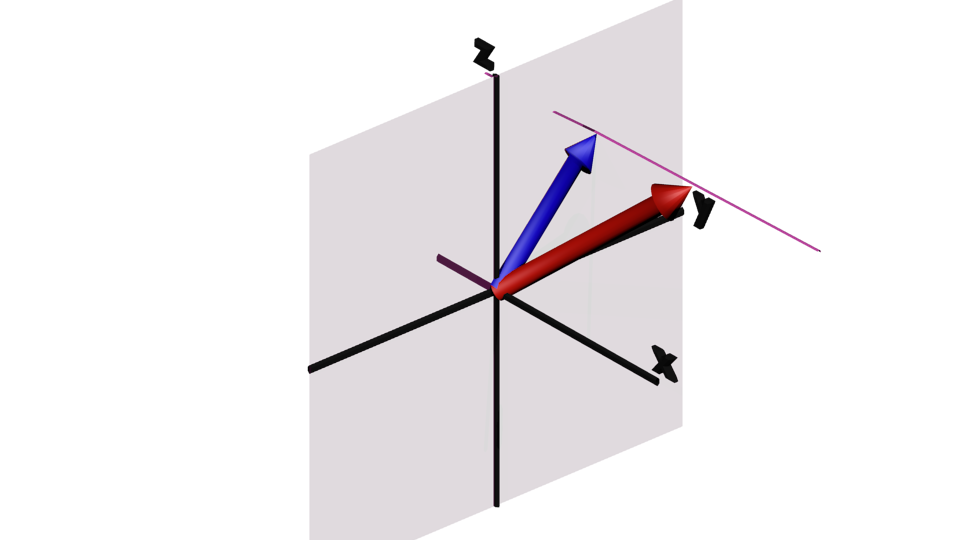
\includegraphics[height=0.7\textheight]{projectionxzPlane}
  }
\end{columns}
\end{frame}

\begin{frame}{Example: Reflection}

  \begin{columns}[T]
    \column{0.3\textwidth}
  Define a matrix transformation by
  \begin{eqnarray*}
    R: & & {\mathbb R}^2 \rightarrow {\mathbb R}^2, \\
    R\vec{x} & = & \twoByTwo{1}{0}{0}{-1}\columnVector{x\\y}.
  \end{eqnarray*}

  \column{0.7\textwidth}

  \dotfield{40}{24}

\end{columns}

\end{frame}

\begin{frame}{Example: Rotation}
  \begin{columns}[T]
    \column{0.34\textwidth}
  Define a matrix transformation by
  \begin{eqnarray*}
    R: & & {\mathbb R}^2 \rightarrow {\mathbb R}^2, \\
    R\vec{x} & = & \twoByTwo{?}{?}{?}{?}\columnVector{x\\y}.
  \end{eqnarray*}

  \column{0.65\textwidth}
  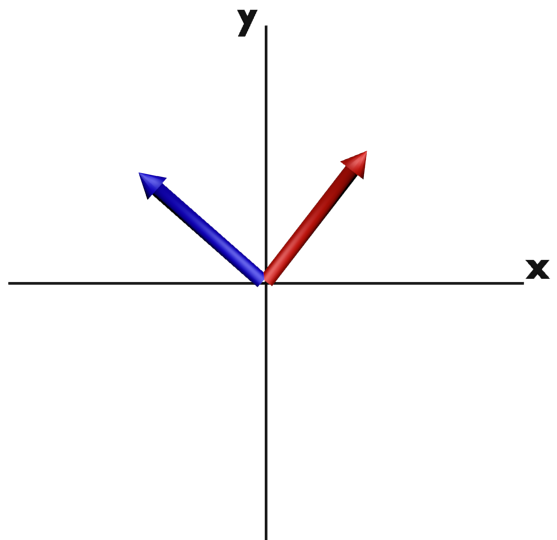
\includegraphics[height=0.7\textheight]{rotatePerp}
\end{columns}
\end{frame}

\begin{frame}{Example: Shear}

  \begin{columns}[T]
    \column{0.5\textwidth}
    \only<1>{\qrcode[height=0.5\textheight]{abcd}}
    \only<2>{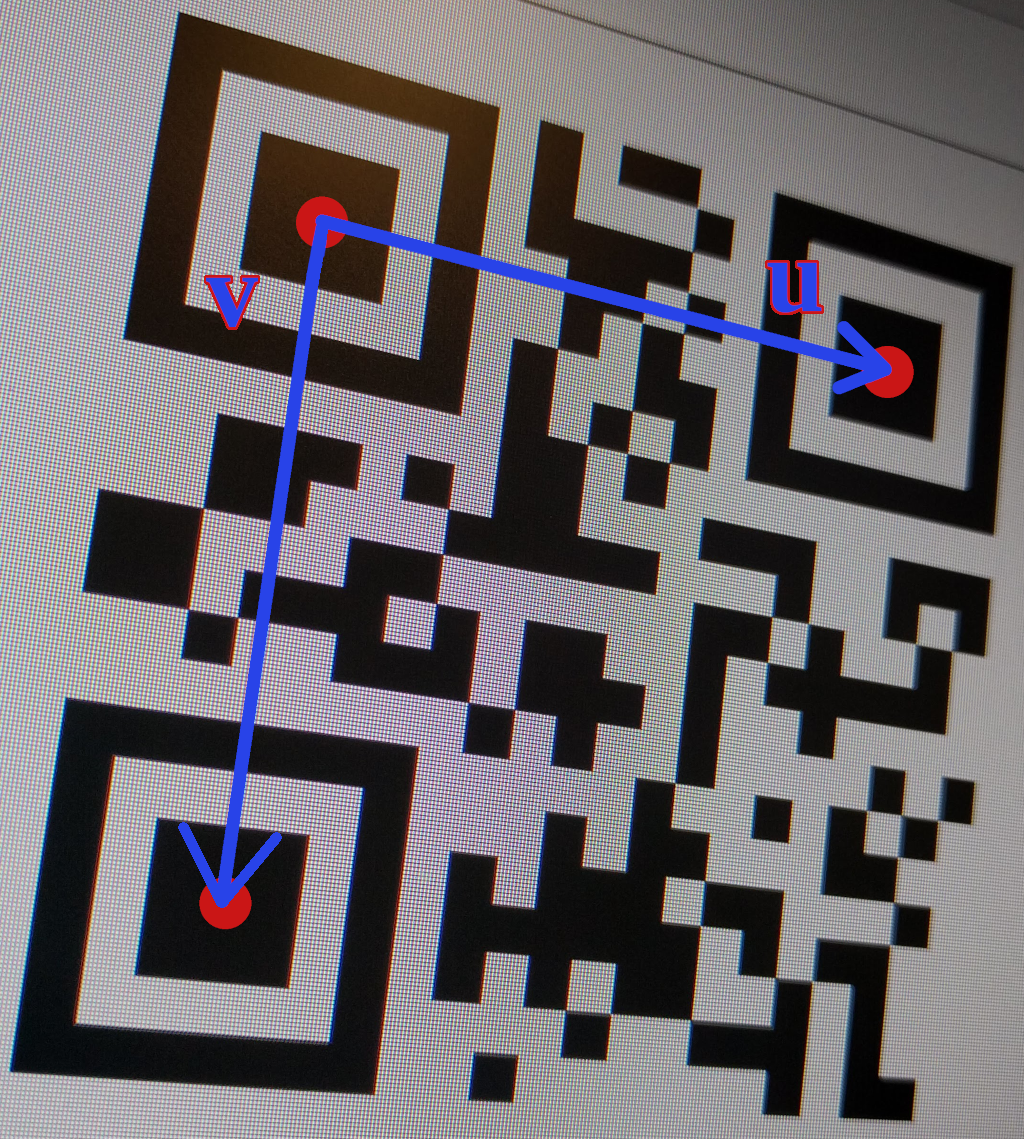
\includegraphics[height=0.7\textheight]{qrCodeSnapshotUV}}
    \column{0.5\textwidth}
    \only<1>{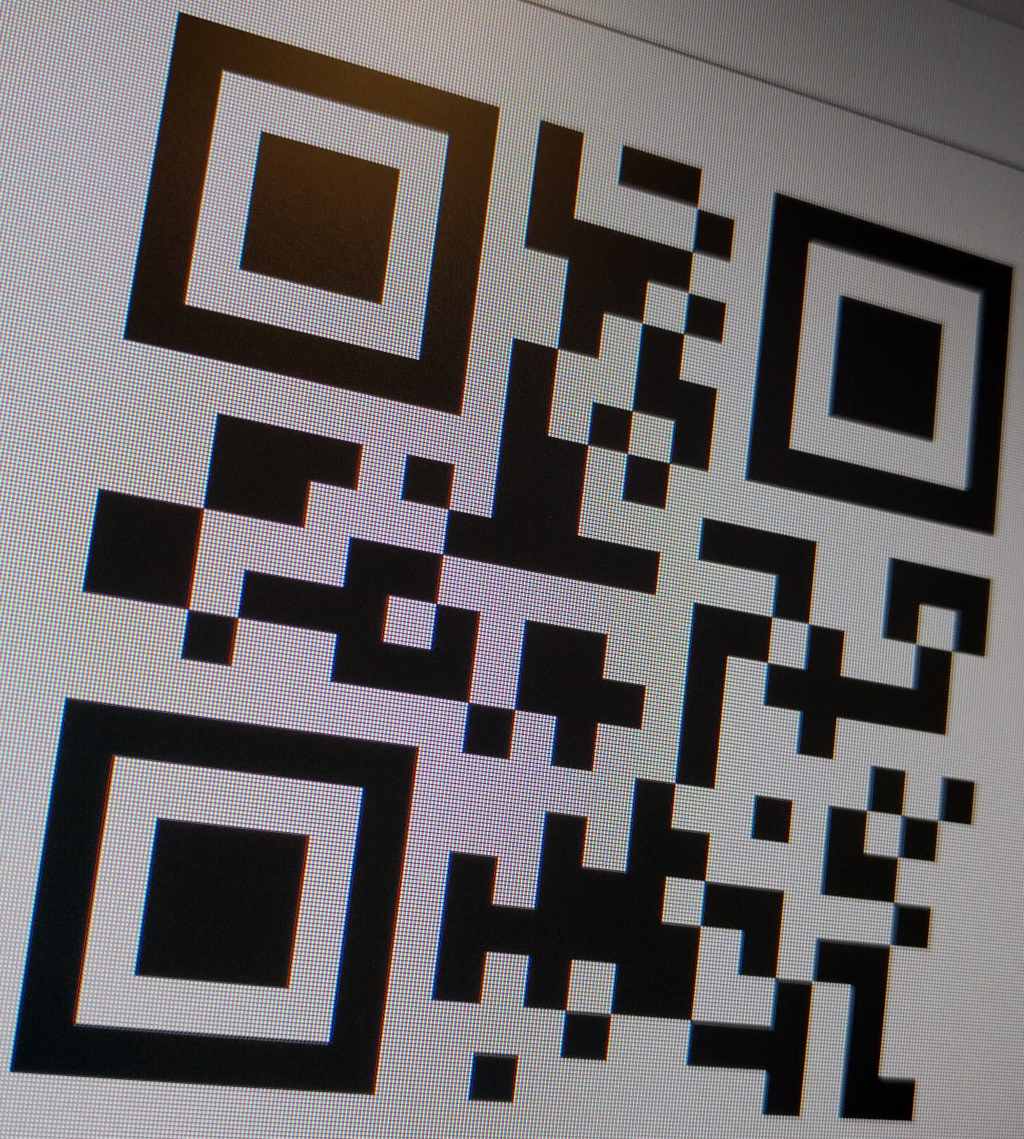
\includegraphics[height=0.7\textheight]{qrCodeSnapshot}}
    \only<2>{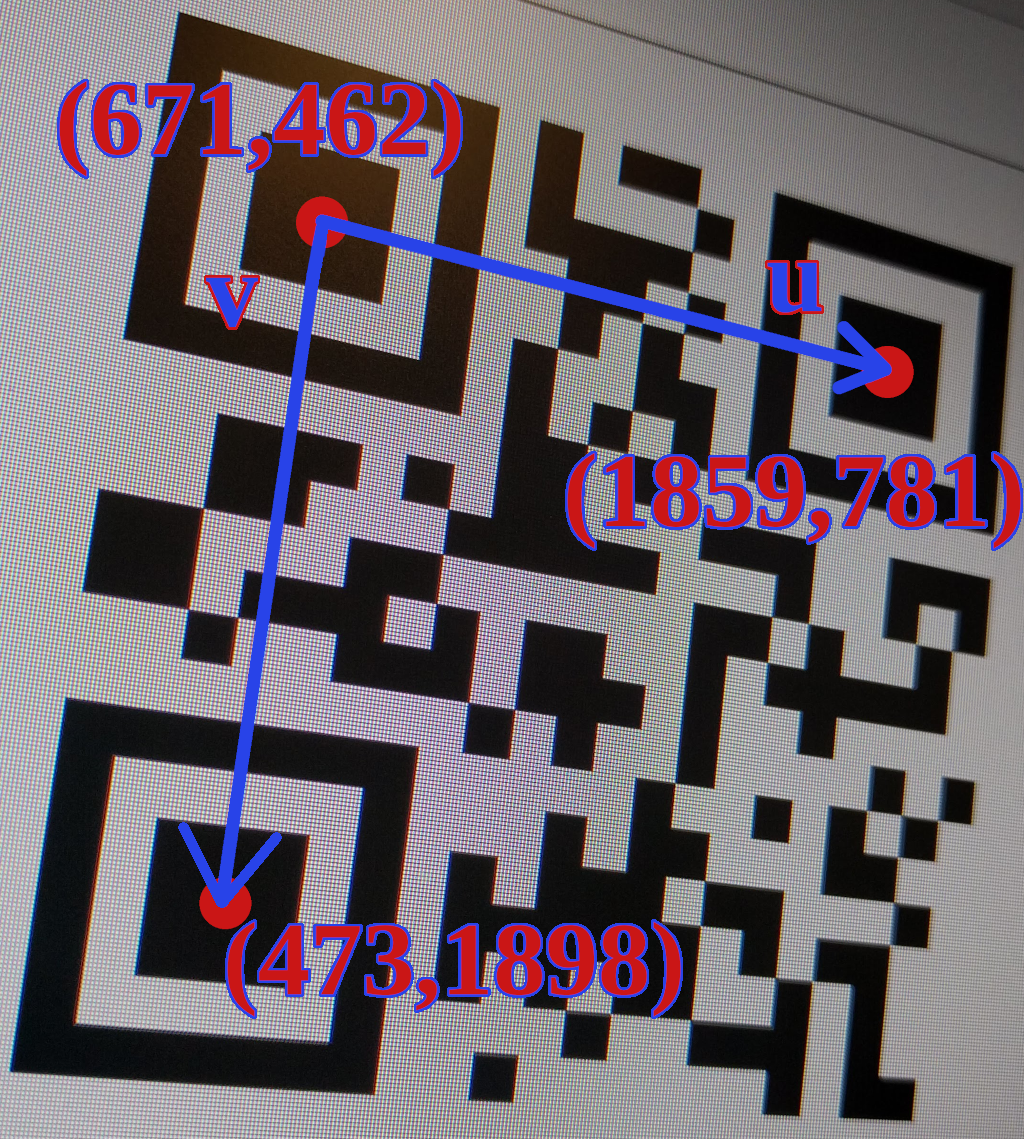
\includegraphics[height=0.7\textheight]{qrCodeSnapshotUV-coordinates}}
\end{columns}
\end{frame}

\begin{frame}{Blank Page}
  \dotfield{60}{24}
\end{frame}


\end{document}
